\documentclass[11pt]{article}

% Packages and stuff
\usepackage{longtable}
\usepackage{listings}
\usepackage[ruled,vlined]{algorithm2e}
\usepackage{algpseudocode}
\usepackage{amssymb}
\usepackage{amsmath}
\usepackage{amsthm}
\usepackage{amsfonts}
\usepackage{booktabs}
\usepackage{enumerate}
\usepackage[shortlabels]{enumitem}
\usepackage{fancyhdr}
\usepackage{fancyvrb}
\usepackage{float}
\usepackage{graphicx}
\usepackage[skins]{tcolorbox}
\usepackage{mathrsfs}
\usepackage{subfig}
\usepackage[hidelinks,pdfauthor = {Maurizio M. Chiaramonte}]{hyperref}
\usepackage{bm}
\usepackage[letterpaper,margin=1in]{geometry}
\usepackage{fancyhdr}
\usepackage[explicit]{titlesec}
%\usepackage{cmbright}
%\renewcommand{\familydefault}{\sfdefault}

%%% Bibliography
\ifcsname#1\endcsname
\ifnum\bibliographynatbib=1
\usepackage[numbers]{natbib}
\bibliographystyle{plainnat}
\else

\usepackage[natbib=true,maxnames=5,style=numeric,maxcitenames=1,firstinits=true,defernumbers,backend=biber,	sorting=none,
    url=false, 
    doi=false,
    eprint=false]{biblatex}
\fi
\else 
\usepackage[natbib=true,maxnames=5,style=numeric,maxcitenames=1,firstinits=true,defernumbers,backend=biber,	sorting=none,
    url=false, 
    doi=false,
    eprint=false]{biblatex}
\fi

\usepackage{multicol}
\usepackage{stmaryrd}
\usepackage{cancel}
\usepackage[utf8]{inputenc} 
\usepackage[T1]{fontenc}  
\usepackage{appendix}

%%tikz 
\usepackage{tikz}
\usetikzlibrary{arrows}
\usetikzlibrary{backgrounds}
\usetikzlibrary{calc}
\usetikzlibrary{decorations.pathmorphing}
\usetikzlibrary{decorations.pathmorphing}
\usetikzlibrary{decorations.markings}
\usetikzlibrary{decorations.pathreplacing}
\usetikzlibrary{decorations.text}

\usetikzlibrary{external}
\tikzexternalize[prefix=tikz/]
\tikzexternaldisable

\usetikzlibrary{positioning}
\usepackage{pdftexcmds}
\usetikzlibrary{positioning}
\usetikzlibrary{shapes}
\usetikzlibrary{spy}

\usetikzlibrary{knots}

\usetikzlibrary{mindmap}
\usetikzlibrary{patterns}

%% pgfplots
\usepackage{pgfplots}
\usepackage{pgffor}
\usepackage{pgfplotstable}
\pgfplotsset{compat=newest}
\usepgfplotslibrary{fillbetween}
\pgfkeys{/tikz/.cd,
  background color/.initial=white,
  background color/.get=\backcol,
  background color/.store in=\backcol,
}
\pgfplotsset{compat = newest}
\pgfplotsset{
    discard if larger/.style 2 args={
        x filter/.code={
          \edef\tempa{\thisrow{#1}}
          \edef\tempb{#2}
					\ifnum\tempa>\tempb
					\def\pgfmathresult{inf}
					\else\fi}
			}
		}
\pgfplotsset{
    discard if not/.style 2 args={
        x filter/.code={
            \edef\tempa{\thisrow{#1}}
            \edef\tempb{#2}
            \ifx\tempa\tempb
            \else
                \def\pgfmathresult{inf}
            \fi
        }
    }
}
\tikzset{
    mark position/.style args={#1(#2)}{
        postaction={
            decorate,
            decoration={
                markings,
                mark=at position #1 with \coordinate (#2);
            }
        }
    }
}
\tikzset{insert node/.style args={#1 at #2}{
    postaction=decorate,
    decoration={
      markings,
      mark= at position #2
        with
        {
         #1
        }
    }
  }
}
\usepgfplotslibrary{patchplots}



\usepackage{chngcntr}
\usepackage{etoolbox}
\usepackage{lipsum}
\newtheoremstyle{mystyle}
    {\topsep}                    % Space above
    {\topsep}                    % Space below
    {\itshape}                   % Body font
    {}                           % Indent amount
    {\scshape}                   % Theorem head font
    {.}                          % Punctuation after theorem head
    {.5em}                       % Space after theorem head
    {}  % Theorem head spec (can be left empty, meaning ‘normal’)\theoremstyle{mystyle}






\makeatletter
\providecommand*{\input@path}{}
\g@addto@macro\input@path{{./}}% append
\makeatother


%\usepackage{cmbright}

% symbols
\newcommand{\rhox}{\tilde\rho}
\newcommand{\Nh}{\tilde N}
% write as text
\newcommand{\mt}[1]{\mathrm{#1}}

\newcommand{\xt}{{\boldsymbol x}_\top} 
\newcommand{\tipindex}{\tau}
% mathcal
\newcommand{\Ac}{\mathcal{A}}
\newcommand{\Bc}{\mathcal{B}}
\newcommand{\Cc}{\mathcal{C}}
\newcommand{\Dc}{\mathcal{D}}
\newcommand{\Ec}{\mathcal{E}}
\newcommand{\Fc}{\mathcal{F}}
\newcommand{\Gc}{\mathcal{G}}
\newcommand{\Hc}{\mathcal{H}}
\newcommand{\Ic}{\mathcal{I}}
\newcommand{\Jc}{\mathcal{J}}
\newcommand{\Lc}{\mathcal{L}}
\newcommand{\Kc}{\mathcal{K}}
\newcommand{\Mc}{\mathcal{M}}
\newcommand{\Nc}{\mathcal{N}}
\newcommand{\Oc}{\mathcal{O}}
\newcommand{\Vc}{\mathcal{V}}
\newcommand{\Pc}{\mathcal{P}}
\newcommand{\Qc}{\mathcal{Q}}
\newcommand{\qc}{\mathcal{q}}
\newcommand{\Rc}{\mathcal{R}}
\newcommand{\Sc}{\mathcal{S}}
\newcommand{\Tc}{\mathcal{T}}
\newcommand{\Wc}{\mathcal{W}}
% boldface
\newcommand{\alphab}{{\boldsymbol \alpha}}
\newcommand{\betab}{{\boldsymbol \beta}}
\newcommand{\chib}{\boldsymbol \chi}
\newcommand{\vepsb}{\boldsymbol \varepsilon}
\newcommand{\epsb}{\boldsymbol \epsilon}
\newcommand{\etab}{\boldsymbol \eta}
\newcommand{\gammab}{{\boldsymbol \gamma}}
\newcommand{\kpb}{\boldsymbol \kappa}
\newcommand{\lambdab}{{\boldsymbol \lambda}}
\newcommand{\mub}{\boldsymbol \mu}
\newcommand{\omegab}{\boldsymbol \omega}
\newcommand{\pib}{\boldsymbol \pi}
\newcommand{\psib}{\boldsymbol \psi}
\newcommand{\phib}{\boldsymbol \phi}
\newcommand{\taub}{{\boldsymbol \tau}}
\newcommand{\cs}{\boldsymbol \sigma}
\newcommand{\vphib}{\boldsymbol \varphi}
\newcommand{\xib}{{\boldsymbol \xi}}
\newcommand{\Deltab}{\boldsymbol \Delta}
\newcommand{\Omegab}{\boldsymbol \Omega}
\newcommand{\Phib}{{\boldsymbol \Phi}}
\newcommand{\Sigmab}{\boldsymbol \Sigma}
\newcommand{\Thetab}{\boldsymbol \Theta}
\newcommand{\thetab}{\boldsymbol \theta}
\newcommand{\Xib}{\boldsymbol \Xi}
\newcommand{\Pib}{\boldsymbol \Pi}

\newcommand{\1}{{\boldsymbol 1}}
\newcommand{\0}{{\boldsymbol 0}}
\newcommand{\Ab}{{\boldsymbol A}}
\newcommand{\Bb}{{\boldsymbol B}}
\newcommand{\Cb}{{\boldsymbol C}}
\newcommand{\Db}{{\boldsymbol D}}
\newcommand{\Eb}{{\boldsymbol E}}
\newcommand{\Gb}{{\boldsymbol G}}
\newcommand{\Fb}{{\boldsymbol F}}
\newcommand{\Hb}{{\boldsymbol H}}
\newcommand{\Ib}{{\boldsymbol I}}
\newcommand{\Kb}{{\boldsymbol K}}
\newcommand{\Jb}{{\boldsymbol J}}
\newcommand{\Lb}{{\boldsymbol L}}
\newcommand{\Mb}{{\boldsymbol M}}
\newcommand{\Nb}{{\boldsymbol N}}
\newcommand{\Pb}{{\boldsymbol P}}
\newcommand{\Qb}{{\boldsymbol Q}}
\newcommand{\Rb}{{\boldsymbol R}}
\newcommand{\Sb}{{\boldsymbol S}}
\newcommand{\Tb}{{\boldsymbol T}}
\newcommand{\Ub}{{\boldsymbol U}}
\newcommand{\Vb}{{\boldsymbol V}}
\newcommand{\Wb}{{\boldsymbol W}}
\newcommand{\Xb}{{\boldsymbol X}}
\newcommand{\Yb}{{\boldsymbol Y}}
\newcommand{\Zb}{{\boldsymbol Z}}

\newcommand{\ab}{{\boldsymbol a}}
\newcommand{\bb}{{\boldsymbol b}}
\newcommand{\cbold}{{\boldsymbol c}}
\newcommand{\db}{{\boldsymbol d}}
\newcommand{\fb}{{\boldsymbol f}}
\newcommand{\gb}{{\boldsymbol g}}
\newcommand{\jb}{{\boldsymbol j}}
\newcommand{\kb}{{\boldsymbol k}}
\newcommand{\hb}{{\boldsymbol h}}
\newcommand{\lb}{{\boldsymbol l}}
\newcommand{\mb}{{\boldsymbol m}}
\newcommand{\nb}{{\boldsymbol n}}
\newcommand{\pb}{{\boldsymbol p}}
\newcommand{\qb}{{\boldsymbol q}}
\newcommand{\rb}{{\boldsymbol r}}
\newcommand{\sbf}{{\boldsymbol s}}
\newcommand{\tb}{{\boldsymbol t}}
\newcommand{\ub}{{\boldsymbol u}}
\newcommand{\vb}{{\boldsymbol v}}
\newcommand{\wb}{{\boldsymbol w}}
\newcommand{\yb}{{\boldsymbol y}}
\newcommand{\zb}{{\boldsymbol z}}

\newcommand{\ti}{{\text{i}}}
\newcommand{\tj}{{\text{j}}}

% mathbb
\newcommand{\Abb}{\mathbb{A}}
\newcommand{\Ebb}{\mathbb{E}}
\newcommand{\Fbb}{\mathbb{F}}
\newcommand{\Ibb}{\mathbb{I}}
\newcommand{\Cbb}{\mathbb{C}}
\newcommand{\Jbb}{\mathbb{J}}
\newcommand{\Mbb}{\mathbb{M}}
\newcommand{\Nbb}{\mathbb{N}}
\newcommand{\Pbb}{\mathbb{P}}
\newcommand{\Qbb}{\mathbb{Q}}
\newcommand{\Rbb}{\mathbb{R}}
\newcommand{\Sbb}{\mathbb{S}}
\newcommand{\Zbb}{\mathbb{Z}}

% math sans sserif
\newcommand{\Jsf}{\mathsf{J}}

\newcommand{\jsf}{\mathsf{j}}
\newcommand{\nsf}{\mathsf{n }}
\newcommand{\rsf}{\mathsf{r}}
\newcommand{\tsf}{\mathsf{t}}

% math script
\newcommand{\Bsc}{\mathscr{B}}
\newcommand{\Csc}{\mathscr{C}}
\newcommand{\Esc}{\mathscr{E}}
\newcommand{\Fsc}{\mathscr{F}}
\newcommand{\Gsc}{\mathscr{G}}
\newcommand{\Hsc}{\mathscr{H}}
\newcommand{\Psc}{\mathscr{P}}
\newcommand{\Ssc}{\mathscr{S}}
\newcommand{\Vsc}{\mathscr{V}}
\newcommand{\Wsc}{\mathscr{W}}

% Common vectors
\newcommand{\ee}{{ \bf e}}
\newcommand{\EE}{{ \bf E}}
\newcommand{\ve}{{\boldsymbol v}}
\newcommand{\Ve}{{\boldsymbol V}}
\newcommand{\ac}{{\boldsymbol a}}
\newcommand{\x}{{\boldsymbol x}}
\newcommand{\y}{{\boldsymbol y}}
\newcommand{\X}{{\boldsymbol X}}
\newcommand{\tr}{{\bf t}}
\newcommand{\Chi}{{\boldsymbol \chi}}

\newcommand{\msp}[1]{\hbox{\hskip #1in}}
\newcommand{\mmsp}{\hbox{\hskip 0.2in}}
\newcommand{\ephi}{\,{\bf e}_{\varphi}}
\newcommand{\ff}{\,{\bf f}}
\renewcommand{\AA}{\mathbb{ A}}
\newcommand{\QQ}{\mathbb{ Q}}
\renewcommand{\SS}{\mathbb{ S}}
\newcommand{\TT}{\mathbb{ T}}
\newcommand{\ex}{\,{\bf e}_{x}}
\newcommand{\ey}{\,{\bf e}_{y}}
\newcommand{\ethe}{\,{\bf e}_{\vartheta}}
\newcommand{\dethe}{\,\dot{{\bf  e}}_{\vartheta}}
\newcommand{\dephi}{\,\dot{{\bf e}}_{\varphi}}
\newcommand{\epsi}{\,{\bf e}_{\psi}}
\newcommand{\depsi}{\,\dot{{\bf e}}_{\psi}}
\newcommand{\er}{{\,\bf e}_r}
\newcommand{\der}{\,\dot{{\bf e}}_r}
\newcommand{\dder}{\,\ddot{{\bf e}}_r}
\newcommand{\rr}{{\bf r}}

\newcommand{\nn}{{\bf n}}
\newcommand{\erdot}{(\sin(\psi)\dot{\varphi} \ephi + \dot{\psi} \epsi)}
\newcommand{\ephidot}{(-\dot{\varphi} ( \sin(\psi) \er + \cos \psi \epsi))}
\newcommand{\epsidot}{(-\dot{\psi} \er + \cos(\psi) \dot{\varphi} \ephi)}
\newcommand{\Lg}{\mathcal{L}}

% Calculus
\newcommand{\pd}[2]{ \dfrac{\partial #1}{\partial #2}}
\newcommand{\df}[2]{ \frac{d #1}{d #2}}
\newcommand{\mdf}[2]{ \frac{D #1}{D #2}}
\DeclareMathOperator{\cond}{cond}
\DeclareMathOperator{\dive}{div}
\DeclareMathOperator{\supp}{supp}
\DeclareMathOperator{\grad}{grad}
\DeclareMathOperator{\curl}{curl}
\DeclareMathOperator{\Dive}{Div}
\DeclareMathOperator{\Grad}{Grad}
\DeclareMathOperator{\Curl}{Curl}
\DeclareMathOperator{\trace}{\sf tr}
\DeclareMathOperator{\vectorspan}{span}
\DeclareMathOperator{\sign}{sign}
\DeclareMathOperator{\interior}{int}
\DeclareMathOperator{\floor}{floor}
\newcommand{\disc}[1]{\llbracket#1\rrbracket}

% Tensor Notation
\newcommand{\kd}[1]{\delta_{#1}}
\newcommand{\ten}[2]{\ee_#1\otimes\ee_#2}
\newcommand{\id}[2]{\kd{#1#2} \ee_#1\otimes\ee_#2}
\newcommand{\perm}[1]{\varepsilon_{#1}}
\DeclareMathOperator{\sym}{sym}
\DeclareMathOperator{\skews}{skew}

\newcommand{\jacobian}[2]{\mat{3}{\pd{#1_1}{#2_1} \pd{#1_1}{#2_2} \pd{#1_1}{#2_3}\\\pd{#1_2}{#2_1} \pd{#1_2}{#2_2} \pd{#1_2}{#2_3}\\\pd{#1_3}{#2_1} \pd{#1_3}{#2_2} \pd{#1_3}{#2_3}}}

% Box Answer
\newcommand{\boxeq}[1]{%
\vskip 0.5\baselineskip
\noindent\fbox{
\raggedright
\begin{minipage}[l]{\linewidth}
\vskip -0.75\baselineskip
\begin{eqnarray}
#1 
\end{eqnarray}
\end{minipage}
}
\vskip 0.5\baselineskip\noindent
}

% Equation
\newcommand{\eq}[1]{\begin{equation} #1 \end{equation}}
\newcommand{\eqnonumber}[1]{\begin{equation*} #1 \end{equation*}}
\newcommand{\eqa}[2][]{\begin{subequations}#1\begin{eqnarray} #2  \end{eqnarray}  \end{subequations}}
\newcommand{\eqas}[1]{\begin{equation}\begin{split} #1 \end{split} \end{equation}}
\newcommand{\eqax}[1]{\begin{eqnarray*} #1 \end{eqnarray*}}


\newcommand{\vect}[1]{\left\{ \begin{array}{c}#1\end{array}\right\}}
\newcommand{\mat}[2]{\left[ \begin{array}{*{#1}{c}}#2\end{array}\right]}
\newcommand{\br}[1]{\left({#1}\right)}


\newtheorem{theorem}{Theorem}[section]
\newtheorem{lemma}[theorem]{Lemma}
\newtheorem{proposition}[theorem]{Proposition}
\newtheorem{problem}[theorem]{Problem}
\newtheorem{corollary}[theorem]{Corollary}
\newtheorem{assumption}{Assumption}[section]
\usepackage{bm}

\newcommand{\compresslist}{%
\setlength{\itemsep}{1pt}%
\setlength{\parskip}{0pt}%
\setlength{\parsep}{0pt}%
}

\usepackage[nomessages]{fp}

\usepackage{listings}
\lstset{language=python,
    basicstyle=\ttfamily,
    keywordstyle=\bfseries,
	frame = single,
	numbers=right,
	tabsize=2,
}
\usepackage[letterpaper,margin=1in]{geometry}
\usepackage{fancyhdr}
\usepackage[explicit]{titlesec}
%\graphicspath{{./figures/homework_1}} 
%\usepackage{cmbright}
%\renewcommand{\familydefault}{\sfdefault}


\title{PROBLEM SET \#1}

\date{\today}

\author{APC 523/MAE 507/AST 523 : Numerical Algorithms for Scientific Computing \\ Vivek Kumar}

\hypersetup{
pdftitle= {\@title},
pdfauthor = {\@author},
pdfsubject = {},
pdfkeywords = {},
pdfmoddate= {\@date},
pdfcreator = {\@author},
pdftoolbar=true,        
pdfmenubar=true
}
\newcommand{\py}[1]{{\ttfamily #1}}



\makeatletter
\def\@maketitle{
\begingroup
\centering
{
{\Large \MakeUppercase{\@title}\par}
\vskip 0.1\baselineskip
{\normalsize\noindent\@author\par}
\vskip 0.1\baselineskip
{\normalsize\noindent \today \par}
}
\endgroup
}
\makeatother

\titleformat{\section}{\Large}{\MakeUppercase{}\thesection\quad}{0.1em}{{#1}}

\begin{document}

\maketitle

\section{Error in (symmetric) rounding vs chopping}
\textbf{Assertion}: When mapping a real number $x$ to a nearby machine number in $\Rbb(p,q)$, the upper bound in the relative error for symmetric rounding is:
	\begin{align*}
		\left|\frac{x-\mt{rd}(x)}{x}\right|\leq 2^{-p}
	\end{align*}
\textbf{Proof:}\\
Consider the number $x$ to be represented as:
	\begin{align*}
		x = \pm \left(\sum_{l=1}^{\infty} b_{-l}2^{-l}\right)2^e
	\end{align*}
If the number is to be rounded to $p$ terms, two cases arise:
	\begin{itemize}
	\item[] \textbf{CASE I.} The $(p+1)^{\mt{th}}$ is 0.\\
	In this scenario the difference between the true value and the rounded value is given by:
			\begin{align*}
				x - \mt{rd}(x) = \pm\left(\sum_{l=p+2}^{\infty} b_{-l}2^{-l}\right)2^e
			\end{align*}
			The maximum relative error can then be computed as:
			\begin{align*}
				\mt{max}\left|\frac{x-\mt{rd}(x)}{x}\right| 	&= \frac{\mt{max}\left|x-\mt{rd}(x)\right|}{\mt{min}\left|x\right|}\\
																&= \frac{2^{-p-1}2^e}{2^{-1}2^e }\\
																&= 2^{-p}
			\end{align*}
			which is what we set to prove.
	\item[] \textbf{CASE II.} The $(p+1)^{\mt{th}}$ is 1.\\
	In this scenario the maximum difference between the true and the rounded value is obtained as:
			\begin{align*}
				\mt{max}|x - \mt{rd}(x)| = \left(2^{-p} - 2^{-p-1}\right)2^e
			\end{align*}
			This is the case we all the leading terms from $(p+2)$ are $1$. Hence the maximum relative error can be computed as before:
			\begin{align*}
				\mt{max}\left|\frac{x-\mt{rd}(x)}{x}\right| 	&= \frac{\mt{max}\left|x-\mt{rd}(x)\right|}{\mt{min}\left|x\right|}\\
																&= \frac{\left(2^{-p} -2^{-p-1}\right)2^e}{2^{-1}2^e }\\
																&= 2^{-p}
			\end{align*}
			which is what we set to prove
	\end{itemize}
	Both the cases show that the maximum symmetric rounding off error is $2^{-p}$

%
%\section{An accurate implementation of $e^x$}
%\begin{enumerate}[(a)]
%	\item Compute the value of $e^{5.5}$ by working out the terms of the infinite series upto $n=30$ by rounding upto 5-significant figures\\
%			The true value of \py{exp(5.5)} is $244.691932$. Here the data generated is presented here			
%			\begin{table}[H]
%			\centering
%				\begin{tabular}{c|c|c|c|c}
%					$n$ & numerator & denominator & $n^{\mt{th}}$ term & value \\
%					\hline
%					0	&	1.0000	&	1.0000	& 1.0000 & 1.0000\\
%					1 & 5.50000E+00 & 1.00000E+00 & 5.50000E+00 & 6.50000E+00 \\
%					2 & 3.02500E+01 & 2.00000E+00 & 1.51250E+01 & 2.16250E+01 \\
%					3 & 1.66380E+02 & 6.00000E+00 & 2.77300E+01 & 4.93550E+01 \\
%					4 & 9.15090E+02 & 2.40000E+01 & 3.81290E+01 & 8.74840E+01 \\
%					5 & 5.03300E+03 & 1.20000E+02 & 4.19420E+01 & 1.29430E+02 \\
%					6 & 2.76820E+04 & 7.20000E+02 & 3.84470E+01 & 1.67880E+02 \\
%					7 & 1.52250E+05 & 5.04000E+03 & 3.02080E+01 & 1.98090E+02 \\
%					8 & 8.37380E+05 & 4.03200E+04 & 2.07680E+01 & 2.18860E+02 \\
%					9 & 4.60560E+06 & 3.62880E+05 & 1.26920E+01 & 2.31550E+02 \\
%					10 & 2.53310E+07 & 3.62880E+06 & 6.98050E+00 & 2.38530E+02 \\
%					11 & 1.39320E+08 & 3.99170E+07 & 3.49020E+00 & 2.42020E+02 \\
%					12 & 7.66260E+08 & 4.79000E+08 & 1.59970E+00 & 2.43620E+02 \\
%					13 & 4.21440E+09 & 6.22700E+09 & 6.76790E-01 & 2.44300E+02 \\
%					14 & 2.31790E+10 & 8.71780E+10 & 2.65880E-01 & 2.44570E+02 \\
%					15 & 1.27480E+11 & 1.30770E+12 & 9.74840E-02 & 2.44670E+02 \\
%					16 & 7.01140E+11 & 2.09230E+13 & 3.35100E-02 & 2.44700E+02 \\
%					17 & 3.85630E+12 & 3.55690E+14 & 1.08420E-02 & 2.44710E+02 \\
%					18 & 2.12100E+13 & 6.40240E+15 & 3.31280E-03 & 2.44710E+02 \\
%					19 & 1.16660E+14 & 1.21650E+17 & 9.58980E-04 & 2.44710E+02 \\
%					20 & 6.41630E+14 & 2.43300E+18 & 2.63720E-04 & 2.44710E+02 \\
%					21 & 3.52900E+15 & 5.10930E+19 & 6.90700E-05 & 2.44710E+02 \\
%					22 & 1.94100E+16 & 1.12400E+21 & 1.72690E-05 & 2.44710E+02 \\
%					23 & 1.06760E+17 & 2.58520E+22 & 4.12970E-06 & 2.44710E+02 \\
%					24 & 5.87180E+17 & 6.20450E+23 & 9.46380E-07 & 2.44710E+02 \\
%					25 & 3.22950E+18 & 1.55110E+25 & 2.08210E-07 & 2.44710E+02 \\
%					26 & 1.77620E+19 & 4.03290E+26 & 4.40430E-08 & 2.44710E+02 \\
%					27 & 9.76910E+19 & 1.08890E+28 & 8.97150E-09 & 2.44710E+02 \\
%					28 & 5.37300E+20 & 3.04890E+29 & 1.76230E-09 & 2.44710E+02 \\
%					29 & 2.95510E+21 & 8.84180E+30 & 3.34220E-10 & 2.44710E+02 \\
%					30 & 1.62530E+22 & 2.65250E+32 & 6.12740E-11 & 2.44710E+02 \\
%				\end{tabular}
%			\end{table}
%	\item Compute the $e^{5.5}$ using partial sums
%			\begin{itemize}
%				\item The value of $e^{5.5}$ converges to 5-significant digits at $k=18$
%				
%			\end{itemize}
%		
%	\item
%	
%	\item
%\end{enumerate}
%
%\section{Error propagation in exponentiation}
%\begin{enumerate}[(a)]
%	\item Derive the upper bound on relative error resulting from machine arithmetic for the two different algorithms
%		\begin{enumerate}[(i)]
%			\item Multiplying x's one we get:
%				\begin{align*}
%					\mt{fl}\left(x \times x\right) = x^2 (1+\epsilon)
%				\end{align*}
%				By induction, the relative error in computing $x^n$ by repeated multiplication is $\left(1+\epsilon\right)^{n-1}$. If we neglect any terms of type $\Oc\left(\mt{eps}^2\right)$ and higher the error can be written as:
%				\begin{align*}
%				\mt{Relative \ Error} = \br{n-1}\epsilon
%				\end{align*}
%			
%			\item Using exponentiation:
%				\begin{align*}
%					\mt{fl}\br{e^{\mt{fl}\br{n\br{\mt{fl}\br{\mt{ln}x}}}}}	&= \mt{fl}\br{e^{\mt{fl}\br{n\br{\mt{ln}x\br{1+\epsilon_l}}}}}\\
%																			&= \mt{fl}\br{e^{n \mt{ln}x \br{1+\epsilon_l+\epsilon_n}}}\\
%																			&= e^{n \mt{ln}x \br{1+\epsilon_l+\epsilon_n}}\br{1+\epsilon_{\mt{exp}}}\\
%																			&= x^{n\br{1+\epsilon_l+\epsilon_n}}\br{1+\epsilon_{\mt{exp}}}\\
%																			&= x^n\br{x^{n\br{\epsilon_l+\epsilon_n}}\br{1+\epsilon_{\mt{exp}}}}
%				\end{align*}
%		\end{enumerate}
%	\item Suppose $x$ is positive and $a$ is nonzero. Determine the propagated relative error $\epsilon$ in $x^a$ when:
%		\begin{enumerate}[(i)]
%			\item $x$ is an exact machine number  but $a$ is subject to a relative error $\epsilon_a$
%				
%			\item $a$ is an exact machine number  but $x$ is subject to a relative error $\epsilon_x$
%		\end{enumerate}
%		NOTE: Since $a$ is an arbitrary positive number we only focus on the exponentiation method
%\end{enumerate}
%
%\section{Conditioning}
%Consider the function
%	\begin{align*}
%		f(x) = 1 - e^{-x}
%	\end{align*}
%\begin{enumerate}[(a)]
%	\item The condition (cond $f$)($x$) of the function in terms of x is given as:\\
%			\begin{align*}
%			(\mt{cond \ } f)(x)	&= \left|x \frac{f'(x)}{f(x)}\right|\\
%								&= \left|x \frac{e^{-x}}{1-e^{-x}}\right|\\
%								&= \left|\frac{x}{e^x -1}\right|
%			\end{align*}
%		The function $\frac{x}{e^x -1}$ is a monotonically decreasing function between $\left[0,1\right]$ with values being $1$ at $0$ and $0.58$ at $1$. Hence the problem is well conditioned on this interval
%	\item 
%\end{enumerate}
%
%\section{Limits in $\Rbb\left(p,q\right)$}
%
%\begin{enumerate}[(a)]
%	\item The code stopped at $n = 10^{17}$
%	\item The final converged value is $1.0$
%	\item A table of the intermediate values computed for $0 \leq n \leq n_{\mt{stop}}$
%	\begin{table}[H]
%		\centering
%		\begin{tabular}{c|c}
%		n 	& value \\
%		\hline
%		1.0E+00 & 2.0000000000000 \\
%		1.0E+01 & 2.5937424601000 \\
%		1.0E+02 & 2.7048138294215 \\
%		1.0E+03 & 2.7169239322356 \\
%		1.0E+04 & 2.7181459268249 \\
%		1.0E+05 & 2.7182682371923 \\
%		1.0E+06 & 2.7182804690958 \\
%		1.0E+07 & 2.7182816941321 \\
%		1.0E+08 & 2.7182817983474 \\
%		1.0E+09 & 2.7182820520116 \\
%		1.0E+10 & 2.7182820532348 \\
%		1.0E+11 & 2.7182820533571 \\
%		1.0E+12 & 2.7185234960372 \\
%		1.0E+13 & 2.7161100340869 \\
%		1.0E+14 & 2.7161100340870 \\
%		1.0E+15 & 3.0350352065493 \\
%		1.0E+16 & 1.0000000000000 \\
%		1.0E+17 & 1.0000000000000 		
%		\end{tabular}
%	\end{table}
%\end{enumerate}
%The reason why it converges to that value is that the term $\frac{1}{n}$ gets ignored when n reaches $10^{16}$ as the machine epsilon for floating point in python3 is $\approx 10^{-17}$ (This can be tested by computing $0.1+0.1+0.1-0.3$).
%\section{Fun with square roots}
%\begin{figure}[H]
%	\begin{center}
%		\begin{tabular}{c c} %% tabular useful for creating an array of images 
%			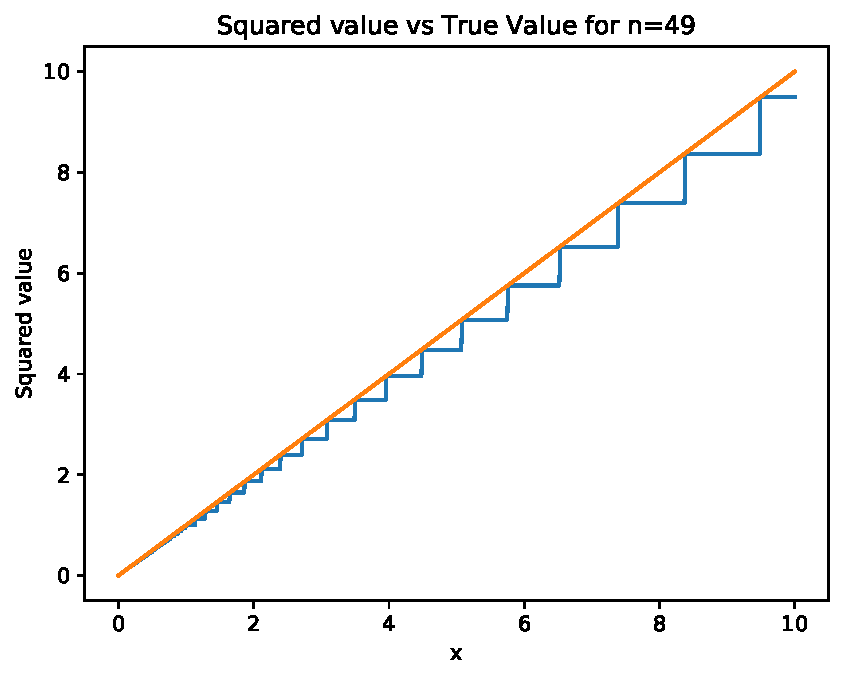
\includegraphics[width=0.45\textwidth]{plot_for_n_49} & 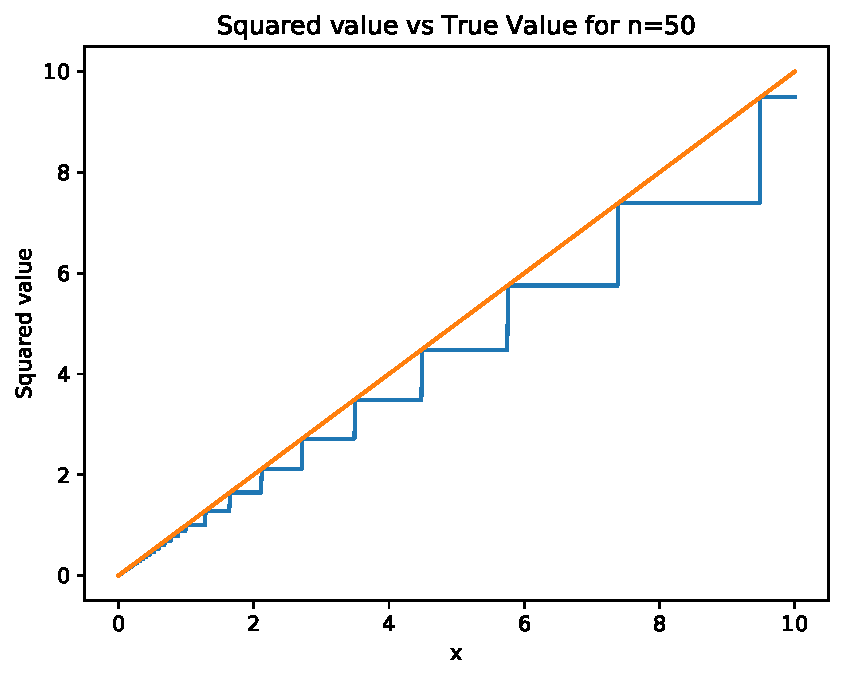
\includegraphics[width=0.45\textwidth]{plot_for_n_50} \\
%			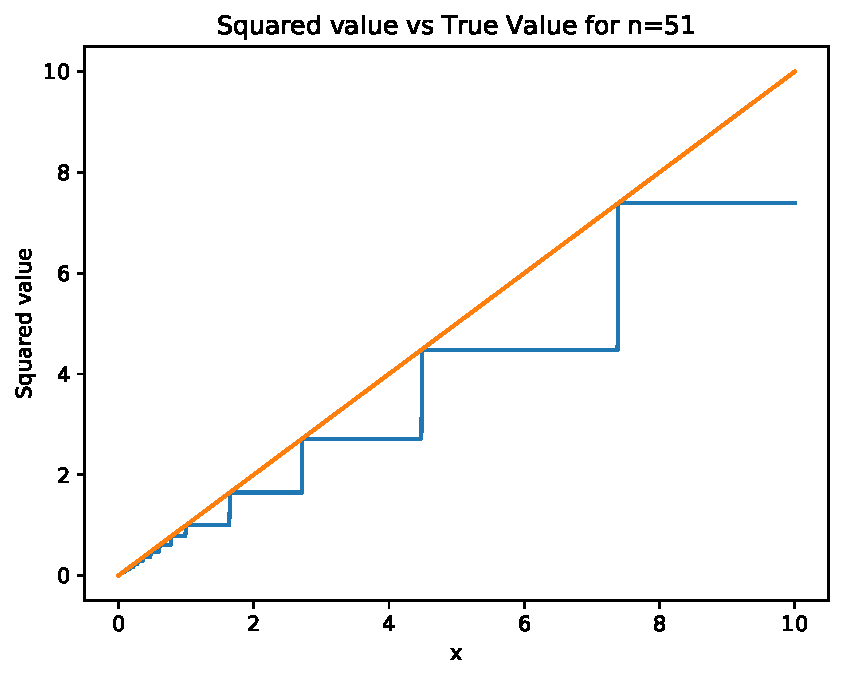
\includegraphics[width=0.45\textwidth]{plot_for_n_51} & 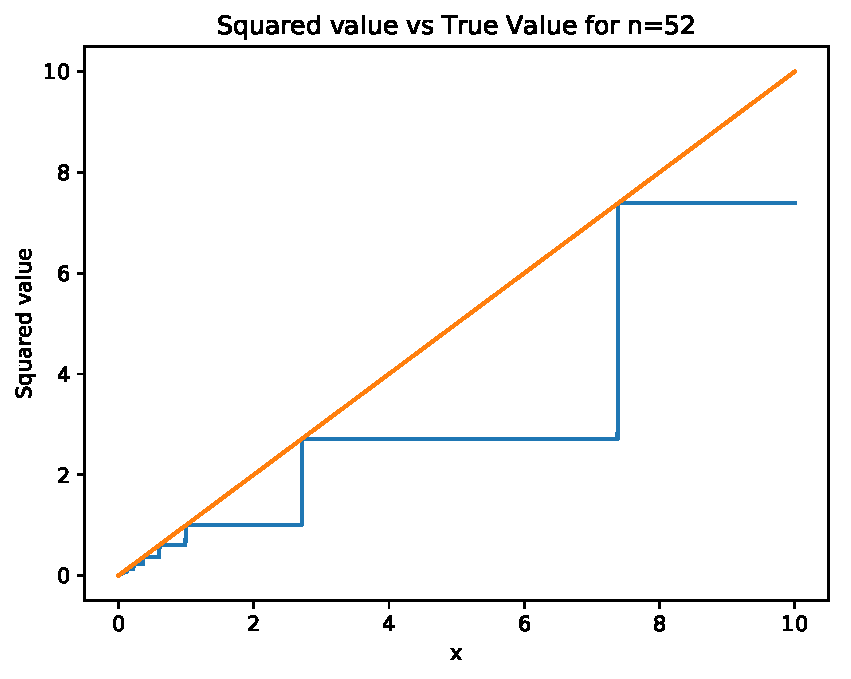
\includegraphics[width=0.45\textwidth]{plot_for_n_52}
%		\end{tabular}
%	\end{center}
%	\caption[funwithsquareroots] 
%	%>>>> use \label inside caption to get Fig. number with \ref{}
%	{ Plots for different values of $n$}
%\end{figure}
%\section{The issue with polynomial roots}
%\begin{enumerate}[(a)]
%	\item The coefficients of the polynomial are:
%		\begin{table}[H]
%			\centering
%			\begin{tabular}{r|r}
%			$n$ & $a_n$\\
%			\hline
%			0	&	2432902008176640000 \\		
%			1	&	-8752948036761600000 \\
%			2	&	13803759753640704000 \\
%			3	&	-12870931245150988800 \\
%			4	&	8037811822645051776 \\
%			5	&	-3599979517947607200 \\
%			6	&	1206647803780373360\\
%			7	&	-311333643161390640\\
%			8	&	63030812099294896\\
%			9	&	-10142299865511450\\
%			10	&	1307535010540395\\
%			11	&	-135585182899530\\
%			12	&	11310276995381\\
%			13	&	-756111184500\\
%			14	&	40171771630\\
%			15	&	-1672280820\\
%			16	&	53327946\\
%			17	&	-1256850\\
%			18	&	20615\\
%			19	&	-210\\
%			20	&	1
%			\end{tabular}
%		\end{table}
%	\item Yes, The newton raphson method converges to $20.00003189$ when the initial guess of $21$ is provided.\\
%			Using the inbuilt function the largest root obtained is $20.00054209$, which is pretty much the same.Further various complex roots are calculated using the inbuilt function
%	\item Changing the coefficient $a_{20}$ from $1 \rightarrow 1+\delta$
%		\begin{table}[H]
%			\centering
%			\begin{tabular}{c|c|c}
%				$\delta$ 	& Largest root using NR & Largest root using inbuilt function \\
%				\hline
%				$10^{-8}$	& $9.5854$ 	& 	$20.648+1.1869j$\\
%				$10^{-6}$	& $7.7527$	&	$23.149 +2.7410j$\\
%				$10^{-4}$	& $5.9693$	&	$28.400 +6.5104j$\\
%				$10^{-2}$	& $5.4696$	&	$38.478 +20.834j$
%			\end{tabular}
%		\end{table}
%	\item Changing the value of coefficient $a_{19}$ from $-210 \rightarrow -210-2^{-23}$
%	\item Consider a monic degree-$n$ polynomial
%\end{enumerate}
%\section{Recurrence in reverse}



\end{document}


